\chapter{Problemanalyse}
\textit{I dette kapitel analyses problemstillinger, som opstår i forbindelse med lægemiddelskift. Disse problemstillinger vil sammenfattes i en opsummering og afsluttes med en problemformulering, der fremadrettet danner  grundlaget for rapporten.}

\section{Årsager til lægemiddelskift}
Lægemiddelskift kan forekomme i forbindelse med kontraktskift, bagatelkøb eller restordre~\citep{Amgros2015}. Kontraktskift kan forekomme ved at lægemidlerne sendes i udbud, såkaldt amgrosudbud. Udbuddene forekommer hvis der findes mere end én leverandør af lægemidlet. Lægemidlerne bringes derved i konkurrence, hvilket kan give anledning til kontraktskift. I tilfælde af patent på lægemidlet, hvormed der kun findes én leverandør, er der ofte ikke konkurrence, da prisen på lægemidlet allerede er fastsat.~\citep{Amgros2015} 

En gang årligt omkring maj eller juni publiceres bagatelkøb af amgros, hvilket kan forårsage lægemiddelskift~\citep{Amgros2018}. I disse tilfælde modtager Amgros pristilbud fra leverandørere med henblik på økonomiske besparelser på lægemiddlerne~\citep{Amgros2012}. I disse tilfælde er Sygehusapoteket er ikke forpligtet til at anvende lægemidlet og leverandøren omfattes ikke af indkøbs- eller forsyningspligt, som ved kontraktskift~\citep{Amgros2018}

Restordre forekommer når efterspørgslen på et lægemiddel overstiger den tilgængelige mængde.~\citep{Amgros2015}. Dette kan f.eks. ske ved leveringesvigt fra leverandøren eller producenten på det ønskede lægemiddel~\citep{Amgros2017, Laegemiddelinformaion2017}. Leveringesvigt skyldes som ofte at producenten har mangel på råvarer eller produktionsvanskeligheder~\citep{Amgros2017, Laegemiddelinformaion2017}. I tilfælde  af restordre er det leverandørens ansvar at dække hospitalsapotekernes udgift ved indkøb af et erstatningslægemiddel\fxnote{KILDE}. 

%\fxnote{\url{https://levportal.amgros.dk/SiteCollectionDocuments/1.\%20Grundl\%C3\%A6ggende\%20information\%20om\%20l\%C3\%A6gemiddeludbud.pdf}}.
 
%I disse tilfælde er sygehusapoteket ikke forpligtet til at anvende lægemidlet og leverandøren omfattes ikke af indkøbs- eller forsyningspligt.~\citep{Amgros2018}Amgros publicerer hvert år i maj/juni udbud for en række lægemidler med en mindre omsætning, der ligger under tærskelværdierne, men som kan have grænseoverskridende interesse. Derfor udbyder vi disse indkøb efter reglerne for udbud under tærskelværdierne. Det er derudover muligt for leverandører at afgive løbende tilbud på de ATC-koder, der er omfattet af bagatelkøb.

\section{Lægemiddeludbud}
Størstedelen af udbud på lægemidler i ATC-grupper sker en gang årligt fra start september til midt november, hvor udbud på ATC-grupper som indgår i RADS behandlingsvejledninger \fxnote{\url{http://www.rads.dk/behandlingsvejledninger}} sker løbende hen over året.~\citep{Sygehusapoteket2017}

Et udbud kan ske ved to udbudsformer, enten på baggrund af lægemidlets pris, hvilket er tilfældet for de fleste lægemidler, eller ved økonomisk mest fordelagtige udbud, hvor prisen vægtes mod andre kriterier ~\citep{Amgros2018a}. Disse kriterier er opstillet på baggrund af juridiske grundlag og kan f.eks. omfatte emballage, håndtering af lægemidlet ved administration samt patientsikkerhedsmæssige aspekter. Der kan være én eller flere vindere ved hver udbudsform, hvilket medfører fire typer af udbud.~\citep{Amgros2018a} De fire udbudstyper fremgår af figur \ref{fig:TypeUdbud}.

\begin{figure}[H]\centering
	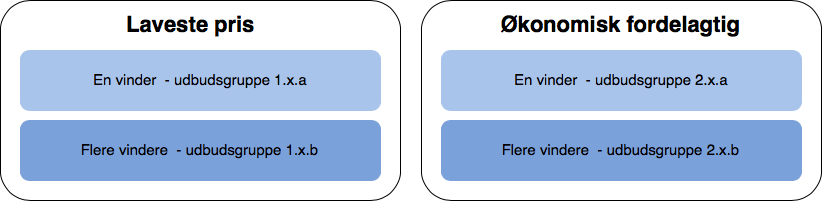
\includegraphics[width=0.7\textwidth]{billeder/TypeUdbud.png} 
	\caption{Udbydstyper.~\citep{Amgros2018a}}
	\label{fig:TypeUdbud}  
\end{figure}

Når et udbud sker indsender ansøgende leverandører en omkostnings- og budgetkonsekvensanalyse for nye lægemidler og indikationer til Medicinrådet~\citep{Amgros2017, Amgros2017a}. Omkostningsanalysen omfatter samfundsomkostninger per patient for den nuværende og den ansøgte behandling.
Budgetkonsekvensanalysen omhandler de samlede økonomiske konsekvenser for regionerne ved at anvende det ansøgte lægemiddel.~\citep{Amgros2017a}

Analyserne vurderes på vegne af Medicinrådet af Amgros i forhold til relevans og valide oplysninger.~\citep{Amgros2017, Amgros2017a} Der vurderes, relevans i klinisk praksis, overholdelse af metodevejledning, kvalitet af omkostningsmodellen og overordnede usikkerheder samt evidensens kvalitet. Yderligere kategoriseres de nye lægemidler og indikationer i forhold til den nuværende behandling i stor, vigtig, lille eller ingen merværdi af Medicinrådet.~\citep{Amgros2017, Amgros2017a}

Den kliniske merværdi og analyserne danner grundlaget for prisforhandling~\citep{Amgros2017, Amgros2017a}. Amgros forhandler med den ansøgende leverandør for at opnå retfærdigt forhold mellem merværdi og meromkostninger i forhold til den nuværende og ansøgte behandling. Ud fra beslutningsgrundlag på forhandlingerne udarbejder Amgros en anbefaling til Medicinrådet.~\citep{Amgros2017, Amgros2017a}

På baggrund af den indsamlede evidens og resultatet af forhandlingerne foretaget af Amgros beslutter Medicinrådet hvorvidt lægemidlet skal anvendes som standardbehandling.~\citep{Amgros2017a} 

\section{Problematikker ved implementering af lægemiddelskift}
Der er både økonomiske og patientsikkerhedsmæssige konsekvenser ved implementeringen af et lægemiddelskift om det skyldes kontraktskift eller restorde~\citep{Amgros2015}. Sværhedsgraden af implementeringen kategoriseres som simpel eller kompleks på baggrund af flere faktorer som f.eks. hvem skiftet har betydningen for, om der er nogle begrænsninger for hvornår et skift kan finde sted og risikovurdering af hvordan det påvirker afsnittet~\citep{Sygehusapoteket2017b}.

Et simpelt lægemiddelskift er vurderet til at påvirke klinikken i lav grad og varetages ofte af logistik-afdeling, hvorimod et kompleks lægemiddelskift påvirker klinikken i mellem til høj grad, hvorfor flere interessenter involveres ved disse skift.~\citep{Laegemiddelinformaion2017,Sygehusapoteket2017a}. 

Simple lægemiddelskift sker til dagligt i forbindelse med at et lægemiddel skiftes, på grund af restordre, til et simpel generisk lægemiddel~\citep{Laegemiddelinformaion2017}. De komplekse skift sker i forbindelse med ændringer af generiske lægemidler som f.eks. styrke, disponeringsform og ændring i hjælpestoffer. Ofte kontaktes interessenter som medicinansvarlige, kontraktsygeplejersker eller medicinservicefarmakonomerne i forhold til at undersøge lægemidlets anvendelighed for det pågældende hospitalsafsnit.~\citep{Laegemiddelinformaion2017,Sygehusapoteket2017a}

\subsection{Utilsigtede hændelser}
I forbindelse med disse skift kan der opstå tilsigtede hændelser (UTH'er)~\citep{Amgros2015}. De hyppigste årsager til UTH'er på de danske hospitaler skyldes i år 2013 medicinering, hvilket udgjorde 23,97~\%.~\citep{Patientombuddet2013}. Antallet af rapporterede UTH'er i Region Nordjylland er steget med over 36\% fra år 2012 til 2014 ~\citep{Jensen2014}. Ud af 824 rapporterede UTH'er i år 2014 omhandlede 97\% medicinering, 86\% administration af medicin og 41\% at medicinen ikke var givet~\citep{Jensen2014}. 

\subsubsection{Utilsigtede hændelser ved kontraktskift}
De patientsikkerhedsmæssige konsekvenser opstået ved kontraktskift er undersøgt af et norsk studie~\citep{Hakonsen2010}. Interview med 100 sygeplejersker påviste at der opstod fejlmedicinering ved generiske lægemidler. Fejl i ordination og manglende dokumentation af lægemiddelskiftet foretaget af lægen blev opdaget af 46~\% sygeplejersker dagligt, hvorimod sygeplejerskerne altid fik lægemiddelsiftet dokumenteret. Yderligere følte 92~\% af sygeplejerskerne at generiske lægemidler var tidskrævende og 91~\% at disse øgede risikoen for fejl ved disponering.~\citep{Hakonsen2010}. De typiske hændelser ved kontraktskift fremgår af Figur \ref{fig:UTHkontraktskift}.

\begin{figure}[H]\centering
	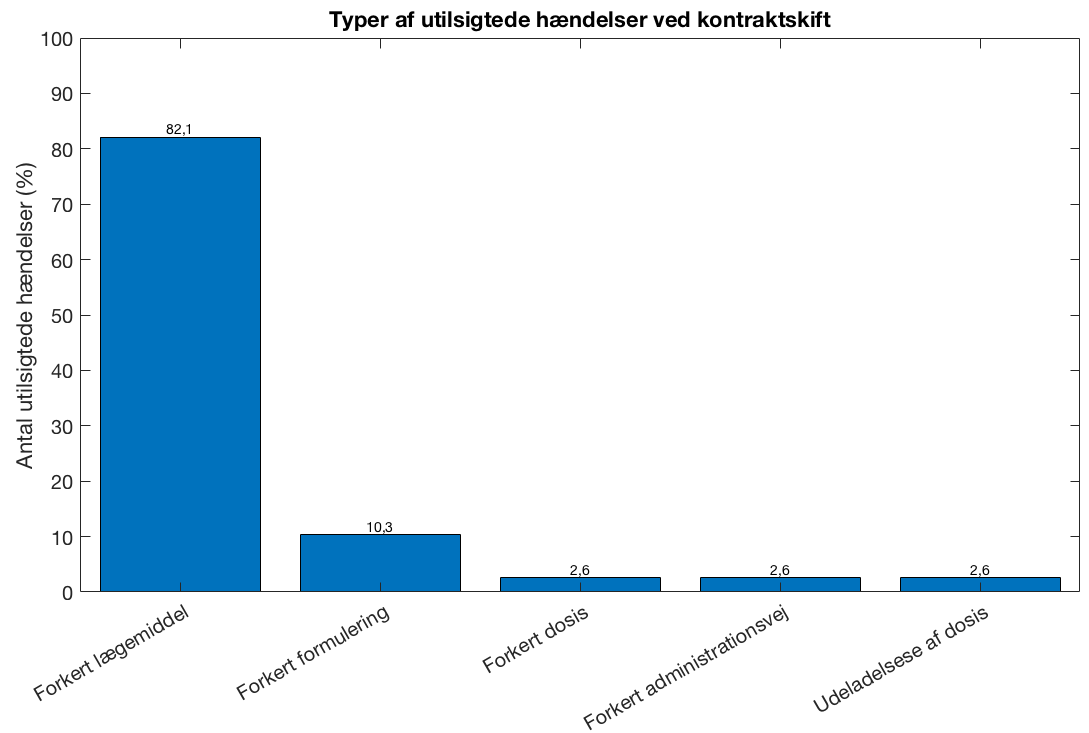
\includegraphics[width=0.7\textwidth]{billeder/UTH1.png} 
	\caption{Utilsigtede hændelser opstået ved kontraktskift\citep{Hakonsen2010}.}
	\label{fig:UTHkontraktskift}  
\end{figure}

Af Figur \ref{fig:UTHkontraktskift} fremgår det at 82,1~\% af UTH'erne forekommer ved disponering af forkert lægemiddel. Den næst hyppigste er forkert formulering hvor 10,3\% af UTH'er er berettiget mod dette. I  sjældnere tilfælde sker forkert dosis, administrationsvej samt udeladelse af dosis. 




\subsubsection{Utilsigtede hændelser ved restordre}
***  Dette afsnit skal ligne afsnittet omkring kontraktskift ***

%*** KIG 3.5.5. Utilsigtede hændelser forårsaget af Restordre *** 16 PDF
%
%De typiske hændelser ved restordre fremgår af Figur \ref{fig:UTHrestordre}.
%
%\begin{figure}[H]\centering
%	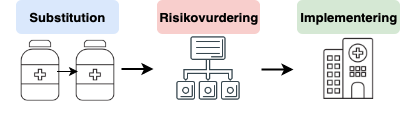
\includegraphics[width=1\textwidth]{billeder/forside.png} 
%	\caption{Utilsigtede hændelser opstået ved restordre\citep{Hakonsen2010}.}
%	\label{fig:UTHRestordre}  
%\end{figure}


\section{Løsninger for problematikker ved lægemiddelskift}

%\subsection{Kontraktskift}

%\subsection{Restordre}
%Disse risici kan mindskes ved instrukser og ændring af procedure på hospitalerne.
%Tæt dialog med leverandøren.
%
%*** SE 19Præparat ***
%
%Jeg skal mere kigge på om det er muligt at gruppere de ting der skal gøres ved lægemiddelskift. Altså vejledninger. 

\section{Opsummering af problemstillinger}
\section{Problemformulering}
\textit{Hvordan kan en algoritme udvikles som et hjælpemiddel til at kategorisere typer af lægemiddelskift med henblik på at synliggøre og kunne vejlede i forhold til problematikker der kan opstå ved lægemiddelskift?}

\textit{Hvordan kan en algoritme udvikles som et hjælpemiddel til at kategorisere lægemiddelskift på baggrund af problematikker der kan opstå ved skiftet med henblik på at kunne vejlede ved vurderingen af et nyt lægemiddelskift?} 
